\section{System Schematic Diagrams}
\begin{landscape}
  \begin{center}
  \begin{figure}[H]
    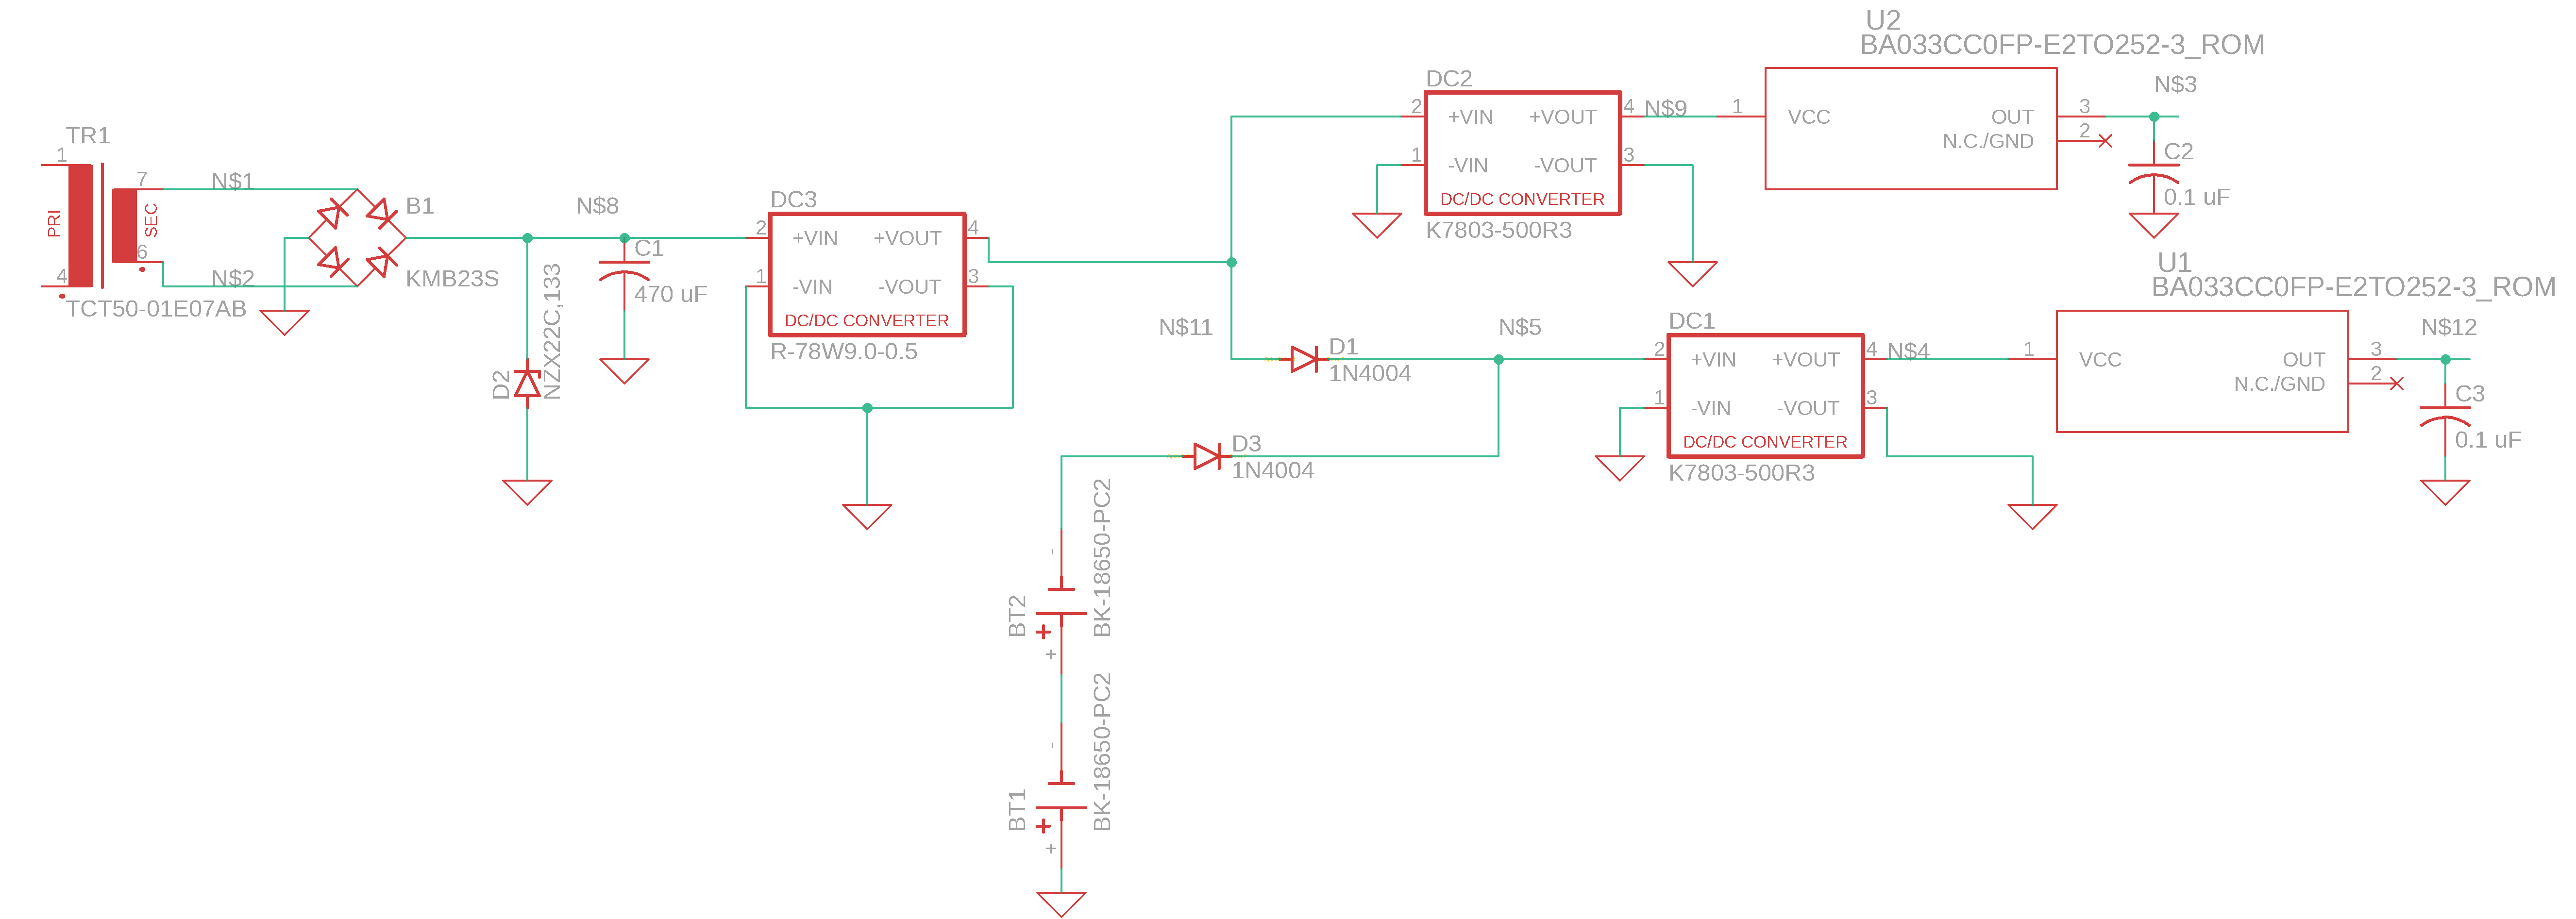
\includegraphics[width=1.6\textwidth, left]{../Power-Supply/Main Unit PSU/main-unit-psu.png}
    \caption{Main Unit PSU Schematic}
    \label{fig:main-psu-schematic}
  \end{figure}
  \end{center}
\createfigurew{../Power-Supply/Sub Unit PSU/sub-unit-psu.png}{Sub Unit PSU Schematic}{fig:sub-psu-schematic}
  \begin{center}
  \begin{figure}[H]
    \includegraphics[width=\pdfpagewidth,height=0.75\textheight]{../Main-Unit/Figures/main-unit.png}
    \caption{Main Unit Schematic}
    \label{fig:main-unit-schematic}
  \end{figure}
  \end{center}
  \begin{center}
  \begin{figure}[H]
    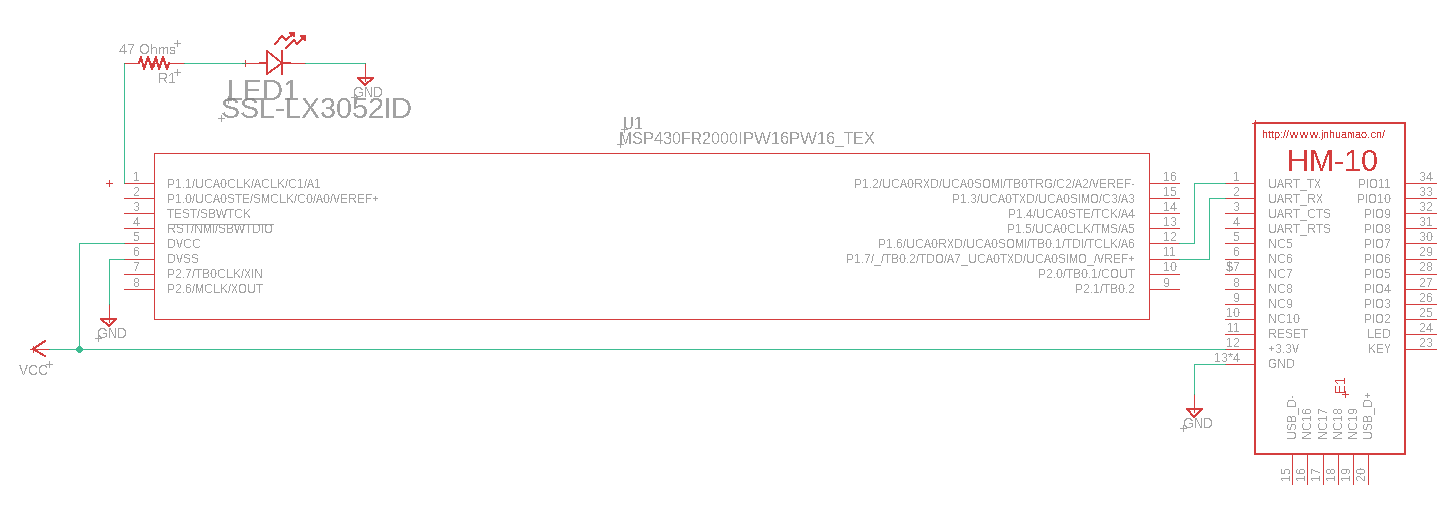
\includegraphics[width=\pdfpagewidth]{../Sub-Unit/Figures/sub-unit.png}
    \caption{Sub Unit Schematic}
    \label{fig:sub-unit-schematic}
  \end{figure}
  \end{center}
  \begin{center}
  \begin{figure}[H]
    
\includegraphics[width=\pdfpagewidth,height=0.65\textheight]{../Main-Unit-and-PSU/Figures/main-unit-and-psu.png}
    \caption{Main Unit with PSU Schematic}
    \label{fig:main-with-psu-schematic}
  \end{figure}
  \end{center}
  \begin{center}
  \begin{figure}[H]
    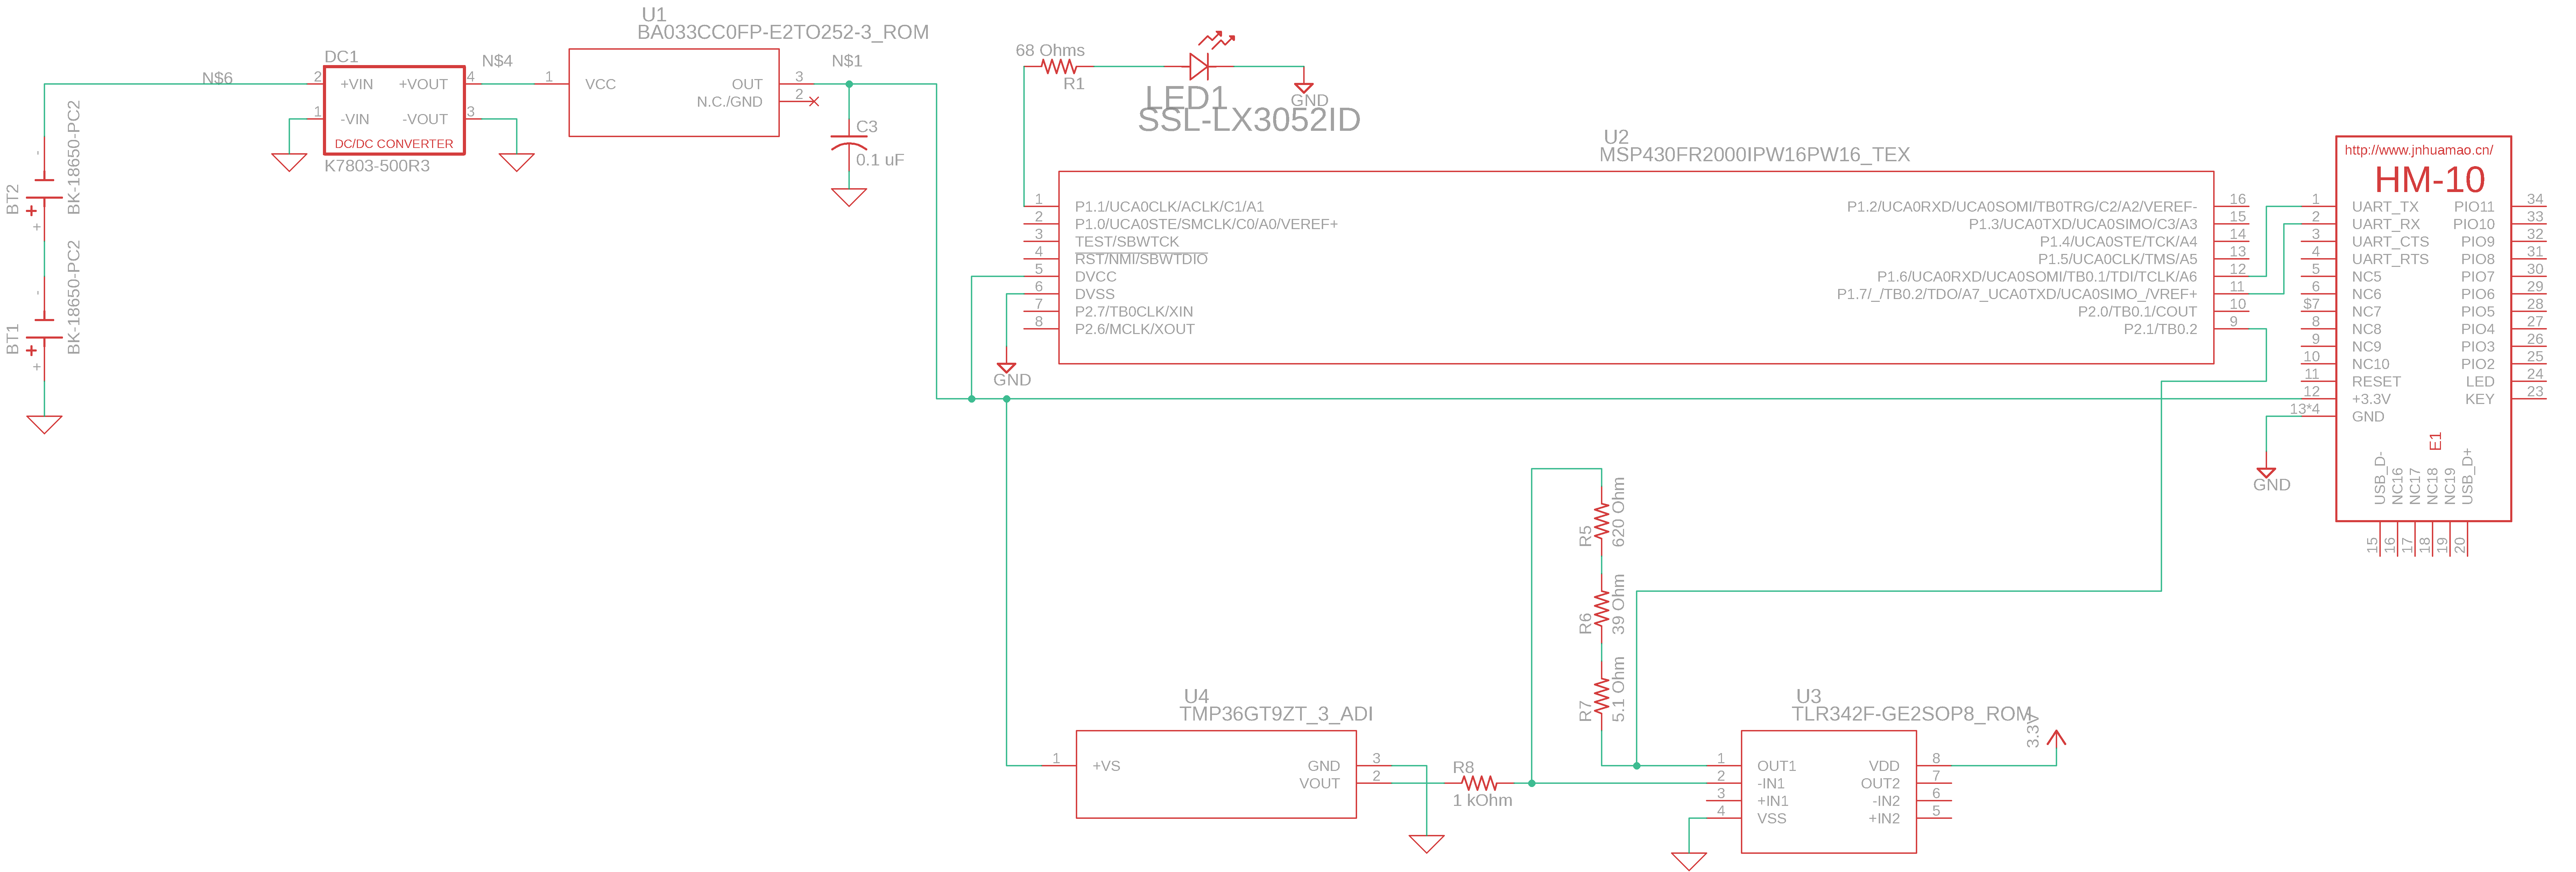
\includegraphics[width=\pdfpagewidth,height=0.65\textheight]{../Sub-Unit-and-PSU/Figures/sub-unit-and-psu.png}
    \caption{Sub Unit with PSU Schematic}
    \label{fig:sub-with-psu-schematic}
  \end{figure}
  \end{center}
\end{landscape}
